\documentclass{article}
\usepackage[top=2cm, bottom=3cm, left=1.5cm, right=1.5cm]{geometry}
\usepackage{amsmath,amsthm}
\usepackage{bm}
\usepackage{color}
\usepackage{graphicx}
\usepackage{epstopdf}
\usepackage{enumitem}
\usepackage{amsfonts}
\usepackage{subcaption}
\usepackage{fourier}
\usepackage{ctex}
\begin{document}
\title{平面几何第一次讲座讲义}
\author{赵丰\footnote{Copyright:Creative Commons Attribution-Share Alike 4.0 International}}
\maketitle
\begin{enumerate}
\item 

如图\ref{fig:Triangle_ABC_with_bisector_AD} 所示,
$\angle BAD = \angle DAC \Leftrightarrow
\frac{BD}{DC}=\frac{AB}{AC}$,此为角平分线定理及其逆定理。

    \begin{figure}[!ht]
    \centering
    \begin{subfigure}[b]{0.45\textwidth}
    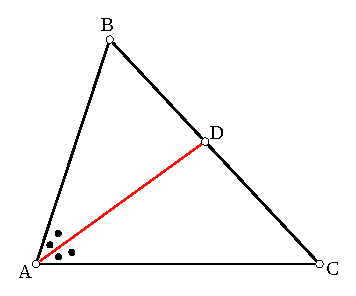
\includegraphics[width=\textwidth]{Triangle_ABC_with_bisector_AD.eps}
    \caption{角平分线定理示意图}\label{fig:Triangle_ABC_with_bisector_AD}
    \end{subfigure}~
    \begin{subfigure}[b]{0.45\textwidth}
    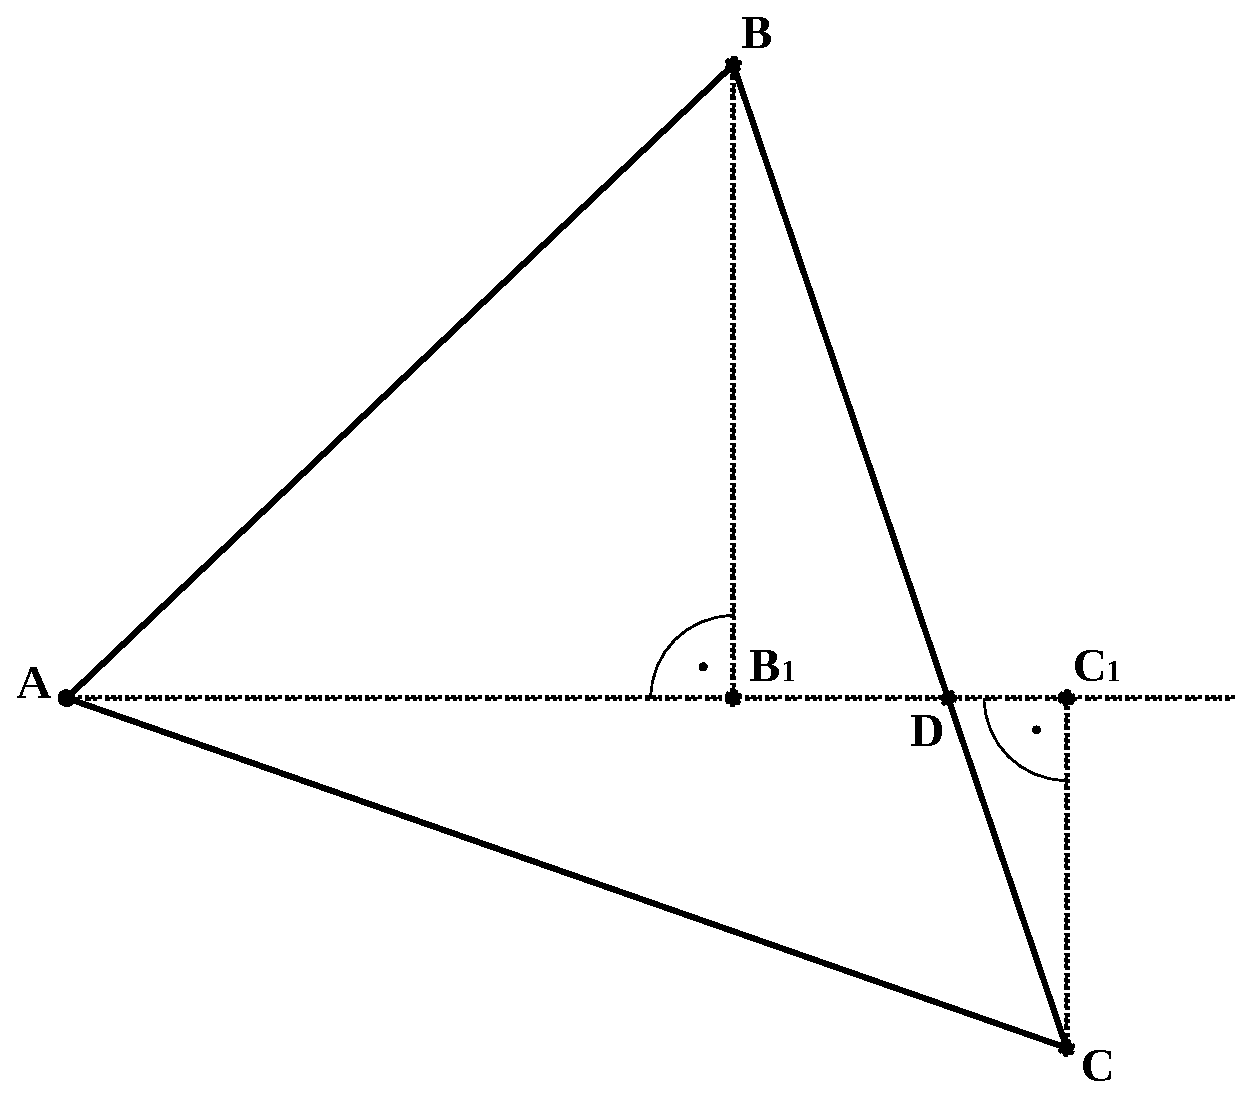
\includegraphics[width=\textwidth]{Bisekt.eps}
    \caption{角平分线证明用图}\label{fig:Bisect}
    \end{subfigure}
    \end{figure}


一般的,去掉$\angle BAD = \angle DAC$的条件,在图\ref{fig:Bisect} 中有:
\[
\frac{BD}{DC}=\frac{AB\sin\angle DAB}{AC \sin\angle DAC}
\]
角平分线逆定理的证明如下:
\begin{proof}[证明]
在图\ref{fig:Bisect} 中,过$B$作$BB_1\perp AD$,垂足为$B_1$; 过$C$作$CC_1 \perp AD$,垂足为
$C_1$。因为$\triangle BB_1D \sim \triangle CC_1D$,所以$\frac{BD}{DC}=\frac{BB_1}{CC_1}$。
因为$\frac{BD}{DC}=\frac{AB}{AC}$,所以$\frac{BB_1}{CC_1}=\frac{AB}{AC}$。
即$\frac{BB_1}{AB}=\frac{CC_1}{AC}\Rightarrow \sin\angle BAD = \sin \angle CAD$。
因为$\angle BAD,\angle CAD$都是锐角,所以$\angle BAD=\angle CAD$。
\end{proof}
\begin{proof}[另证]
$$\frac{BD}{DC}=\frac{S_{\triangle ABD}}{S_{\triangle ADC}}=\frac{AB\cdot AD \cdot \sin\angle BAD}
{AC\cdot AD\cdot \sin\angle DAC}=\frac{AB}{AC}$$
\end{proof}
\textbf{作业:}证明角平分线定理。即在图\ref{fig:Triangle_ABC_with_bisector_AD} 中,已知
$\angle BAD = \angle DAC$,证明$\frac{BD}{DC}=\frac{AB}{AC}$。
\item 如图\ref{fig:Inscribed_angle_theorem4}所示,$TP$是圆$O$的切线,$\angle PTS$ 是弦切角。
有性质$\angle PTS=\angle TAS$
\begin{proof}[证明]
$$
\angle PTS = 90^{\circ}-\angle STO =\frac{1}{2}(180^{\circ}-\angle STO -\angle TSO)=\frac{1}{2}\angle TOS
=\angle TAS
$$
\end{proof}
    \begin{figure}[!ht]
    \centering
    \begin{subfigure}[b]{0.45\textwidth}
    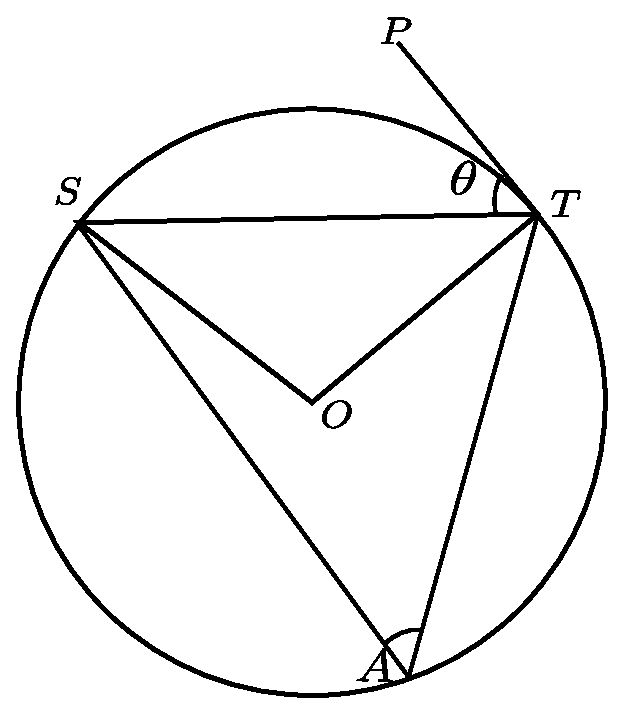
\includegraphics[width=\textwidth]{Inscribed_angle_theorem4.eps}
    \caption{弦切角示意图}\label{fig:Inscribed_angle_theorem4}
    \end{subfigure}~
    \begin{subfigure}[b]{0.45\textwidth}
    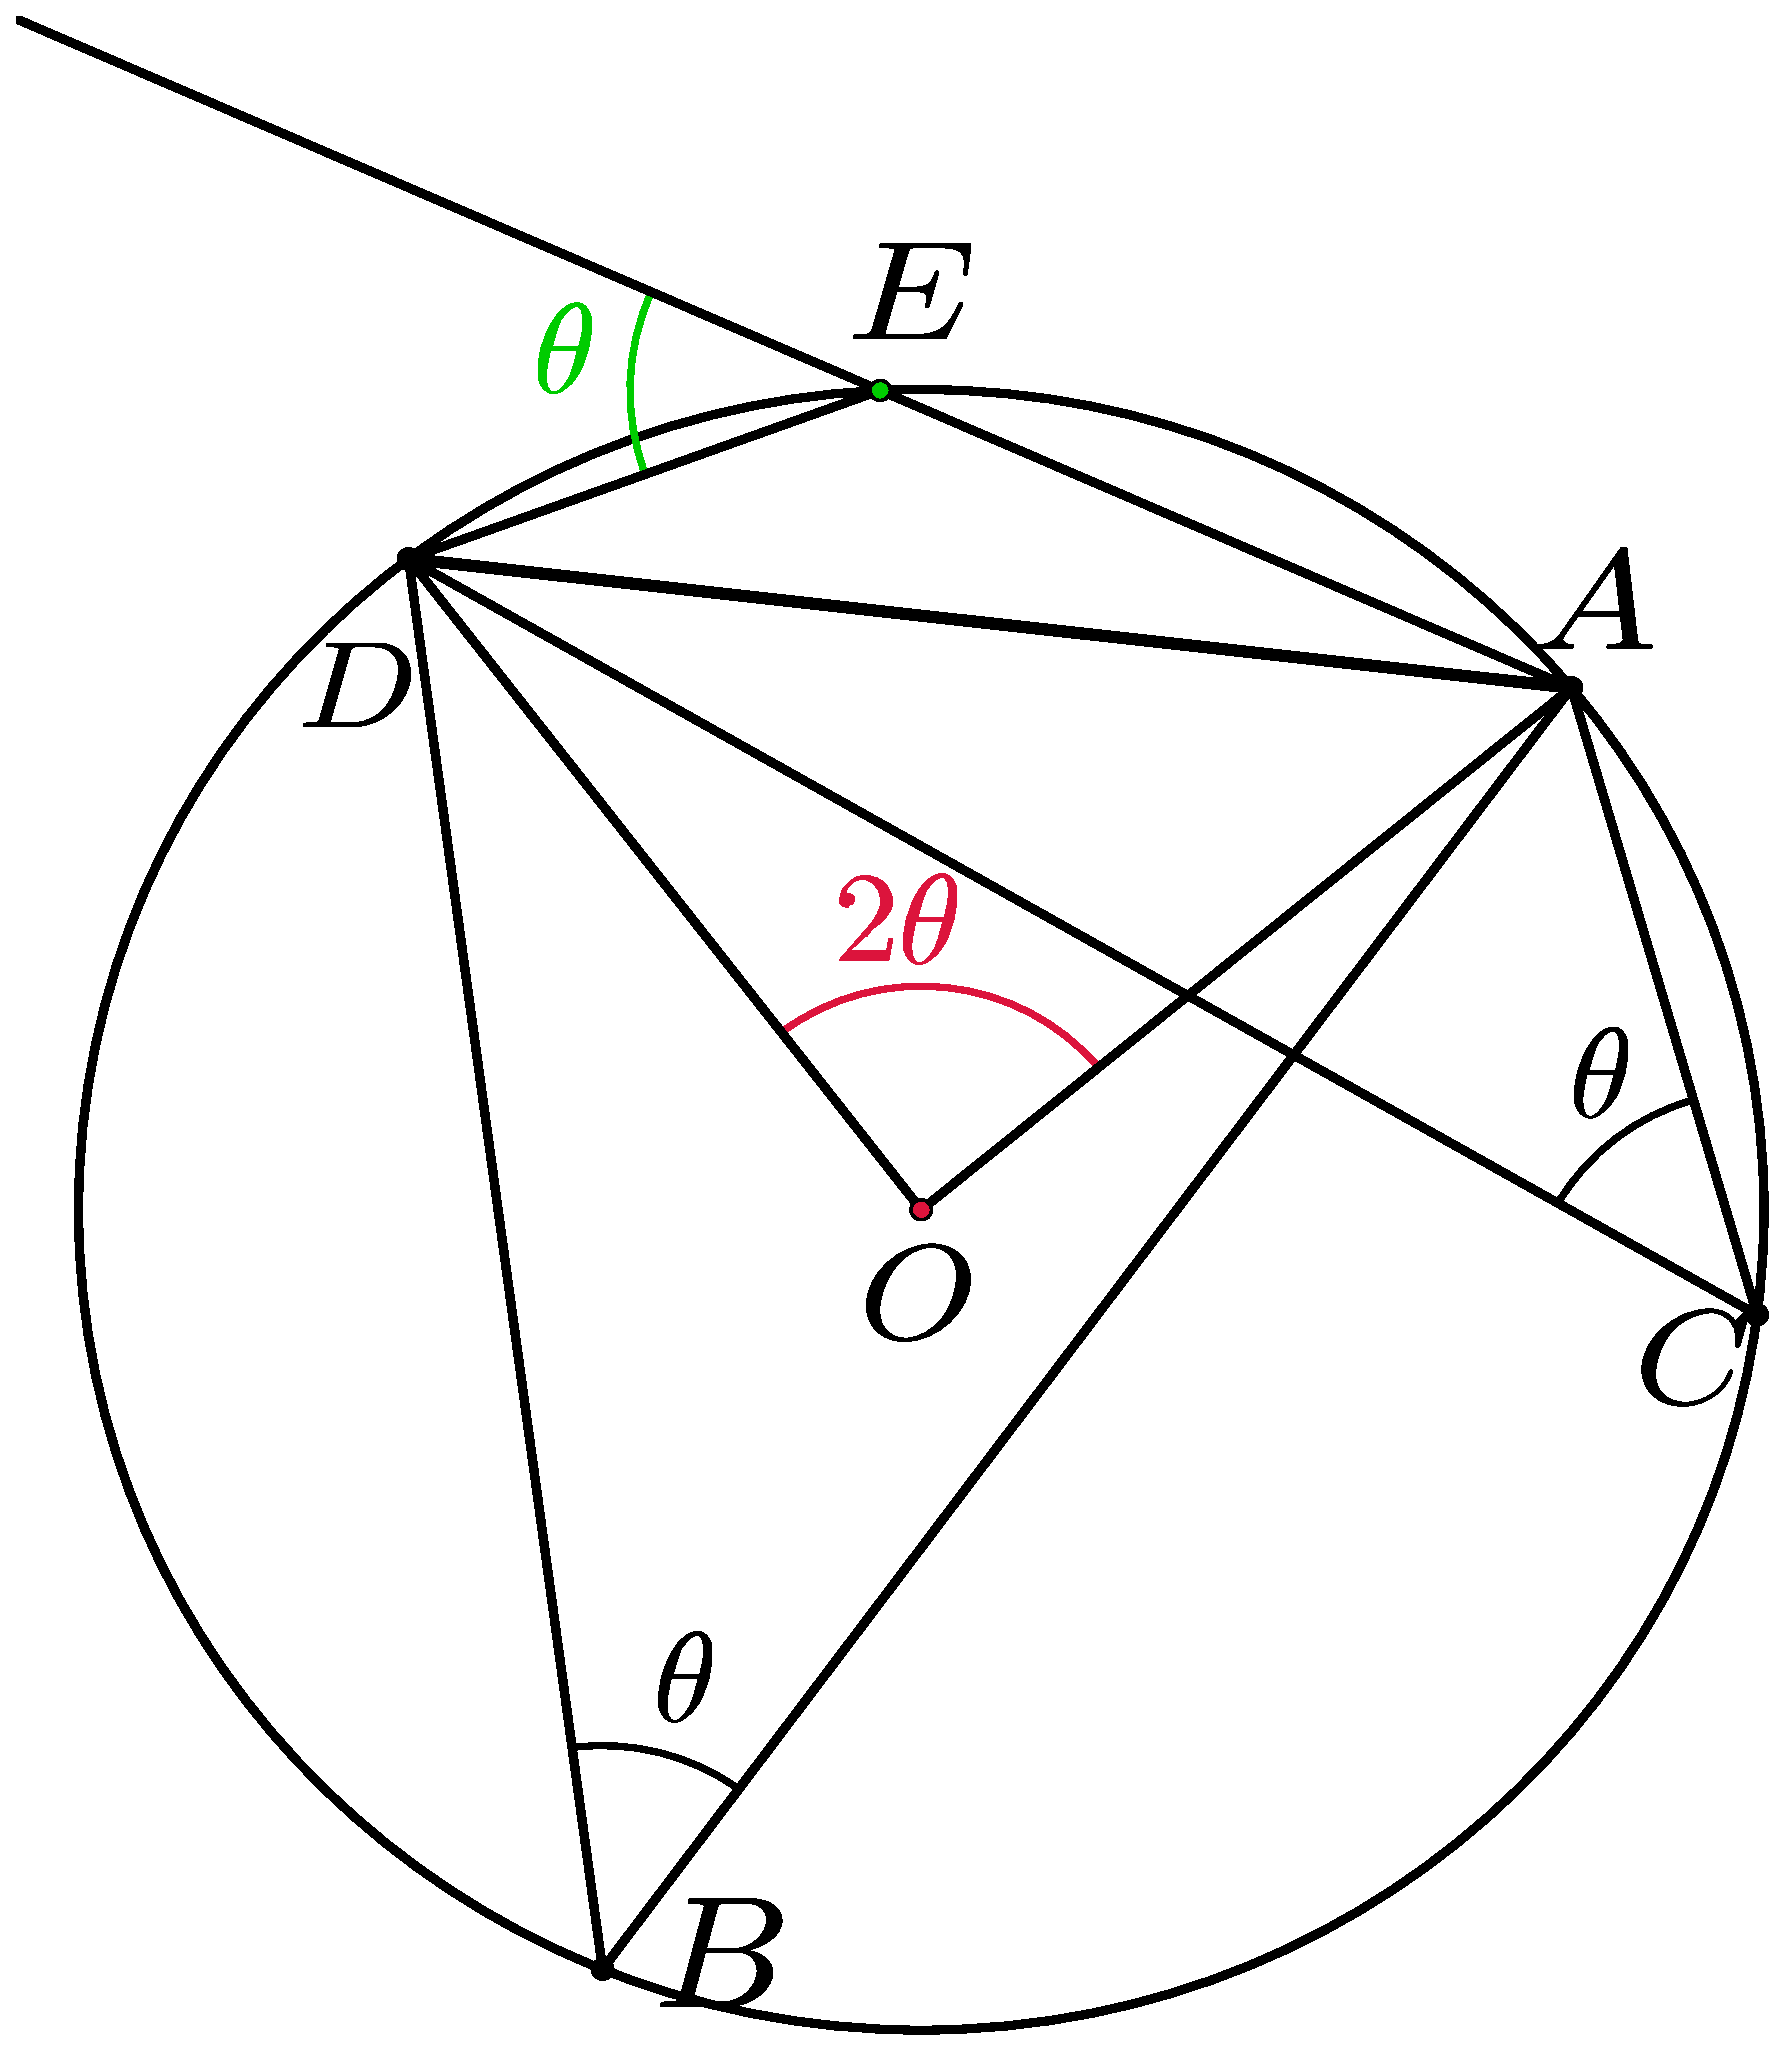
\includegraphics[width=\textwidth]{Inscribed_angles2.eps}
    \caption{四点共圆示意图}\label{fig:Inscribed_angles2}
    \end{subfigure}
    \end{figure}

如图\ref{fig:Inscribed_angles2}所示,$A,B,C,D$四点共圆 $\Leftrightarrow\angle B=\angle C$

并且我们还有: $A,B,D,E$四点共圆 $\Leftrightarrow \angle E=\angle B$ 或者 $\angle B+\angle DEA =180^{\circ}$

练习(\textbf{作业}):
    \begin{figure}[!ht]
    \centering
    \begin{subfigure}[b]{0.31\textwidth}
    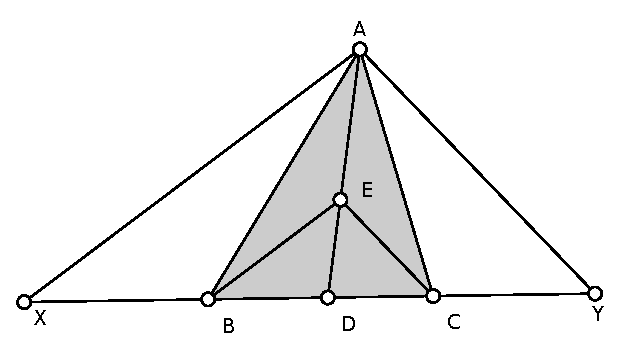
\includegraphics[width=\textwidth]{first_1.eps}
    \caption{角平分线练习题示意图}\label{fig:first_1}
    \end{subfigure}~
    \begin{subfigure}[b]{0.31\textwidth}
    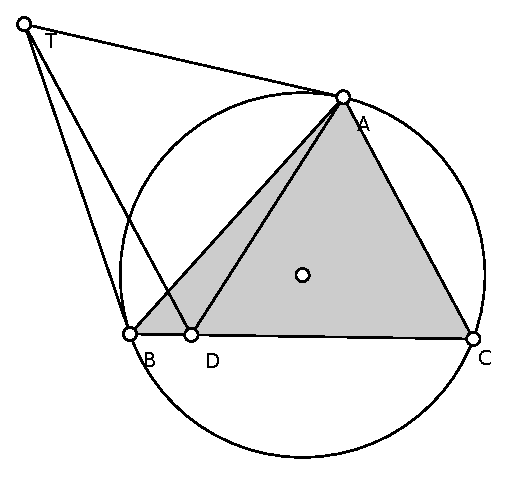
\includegraphics[width=\textwidth]{first_2.eps}
    \caption{弦切角与四点共圆练习题示意图}\label{fig:first_2}
    \end{subfigure}~
    \begin{subfigure}[b]{0.31\textwidth}
    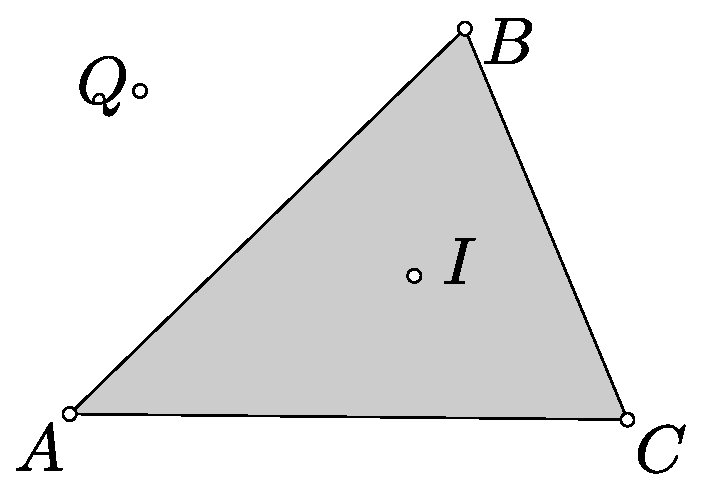
\includegraphics[width=\textwidth]{2018COP_G_P1.eps}
    \caption{综合练习题示意图}\label{fig:2018COP_G_P1}
    \end{subfigure}
    \end{figure}
\begin{enumerate}[label=(\arabic*)]
\item 如图\ref{fig:first_1},$AD$为$\angle BAC$的角平分线,交$BC$于$D$点,$E$为$AD$上一点,过$A$作$BE$的
平行线交$CB$于$X$,作$EC$的平行线交$BC$于$Y$,证明 $BX\cdot AC=CY \cdot AB$。

\item (弦切角与四点共圆综合)如图\ref{fig:first_2},过$A,B$的$\triangle ABC$的切线交于$T$。
过$T$作$TD\parallel AC$交$BC$于$D$,证明$AD=CD$。


\item
(四点共圆)如图\ref{fig:2018COP_G_P1},考虑 $\triangle ABC$, $I$是它的内心,$Q$是$\triangle ABI$的外心,求证 $CIQ$三点共线以及$QACB$四点共圆。
\begin{proof}[证明]
\begin{align*}
&\angle AIB = \angle ACB + \angle IBC + \angle IAC \\
\Rightarrow & \angle QAI + \angle QBI = 2\angle BCI + \angle ABI + \angle BAI \\
\Rightarrow & \angle QAB + \angle QBA = 2\angle BCI \\
\Rightarrow & \angle QAB = \angle BCI = \angle ACI
\end{align*}
所以 $\angle QIA = \angle QAI = \angle QAB + \angle BAI= \angle ACI +\angle IAC$
即 $QIC$三点共线,由$\angle QAB = \angle BCI$易知$QACB$四点共圆。
\end{proof}
\item 
沿用图\ref{fig:2018COP_G_P1},$I$是$\triangle ABC$的内心,延长$CI$交$\triangle ABC$的外接圆于$Q$,
求证$Q$是$\triangle ABI$ 的外心。
\end{enumerate}
\end{enumerate}

\end{document}
